% !TeX root = ../thuthesis-example.tex


\chapter{工业装备状态预测}\label{chapter4}
\section{引言}
本章节介绍了工业装备状态预测的相关内容,包括整体方案的设计,和应用的具体方法,
详细地说明了设计的动机、和实际的效果。

工业装备状态预测的一个重要的应用就是将其应用到预测式故障检测中。

故障检测的一个很直接的思路是,将问题定义成一个分类问题,
分类结果分别是正常和存在故障两种状态,
这样也能通过历史数据训练神经网络模型,得到我们想要的结果。
但是在工业装备状态预测下,
作为分类问题建模存在的问题是样本极度地不平衡。
设备发生故障的情况相对正常情况会很少,
甚至是从来没有出现过故障。
在这样的情况下,分类的难度会特别大。

\begin{figure}
    \centering
    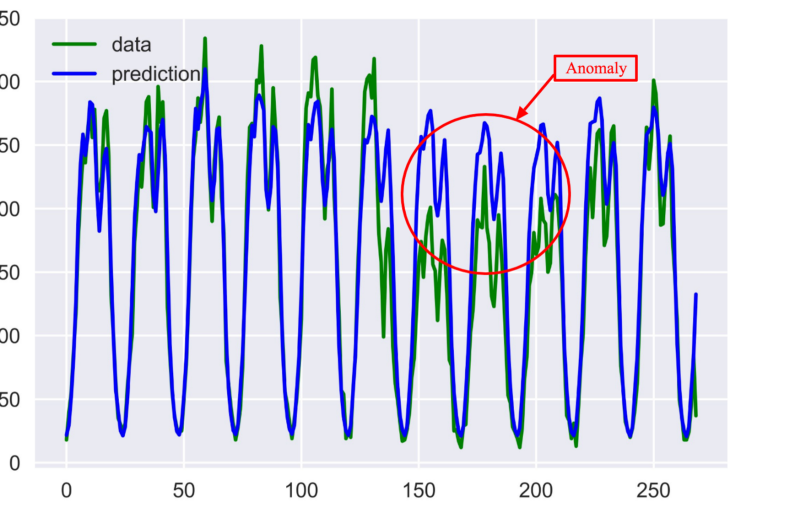
\includegraphics[width=0.6\linewidth]{figures/预测式故障检测}
    \caption{预测式故障检测示意图}
    \label{fig:prediction-fault-detection}
\end{figure}

如图\ref{fig:prediction-fault-detection}中所示,
当实际采集到的工业装备状态数据和预测数据发生较大的偏差时(图中红圈部分),
我们就可以认为是装备发生了故障。
这个前提是需要被检测到的故障会引起相应检测状态的变化,
例如在很多装备或者电子元器件中,
如果发生温度偏离正常运行状态过高,就可以认为是发生了故障。

\begin{figure}
  \centering
  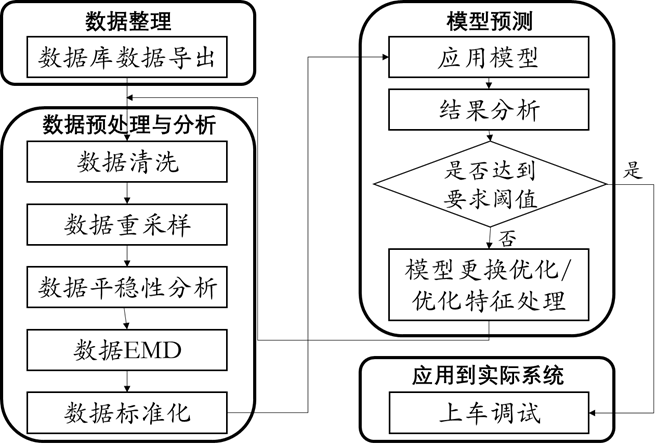
\includegraphics[width=0.8\linewidth]{figures/列车轴温预测系统流程框架图.png}
  \caption{列车轴温预测系统流程框架图}
  \label{fig:prediction_system}
\end{figure}

以列车走行部作为状态预测为例,
可以设计如图\ref{fig:prediction_system}的故障预测系统。
分为数据整理、数据预处理与分析、模型预测、应用到实际系统调试几个模块。

为了能达到能够上车调试的效果,需要对模型进行不断地迭代和优化,
直到预测的效果能够达到某一个特定的阈值。
这部分我们只关注预测的结果,可以和上车调试部分独立出来,成为一个单独的模块。
在下面的部分,我们只讨论工业装备状态预测的部分,
主要关注如何提升预测的效果,减小预测结果和实际结果之间的偏差。

\section{工业装备状态预测方案}
\subsection{系统设计}

  \begin{figure}
    \centering
    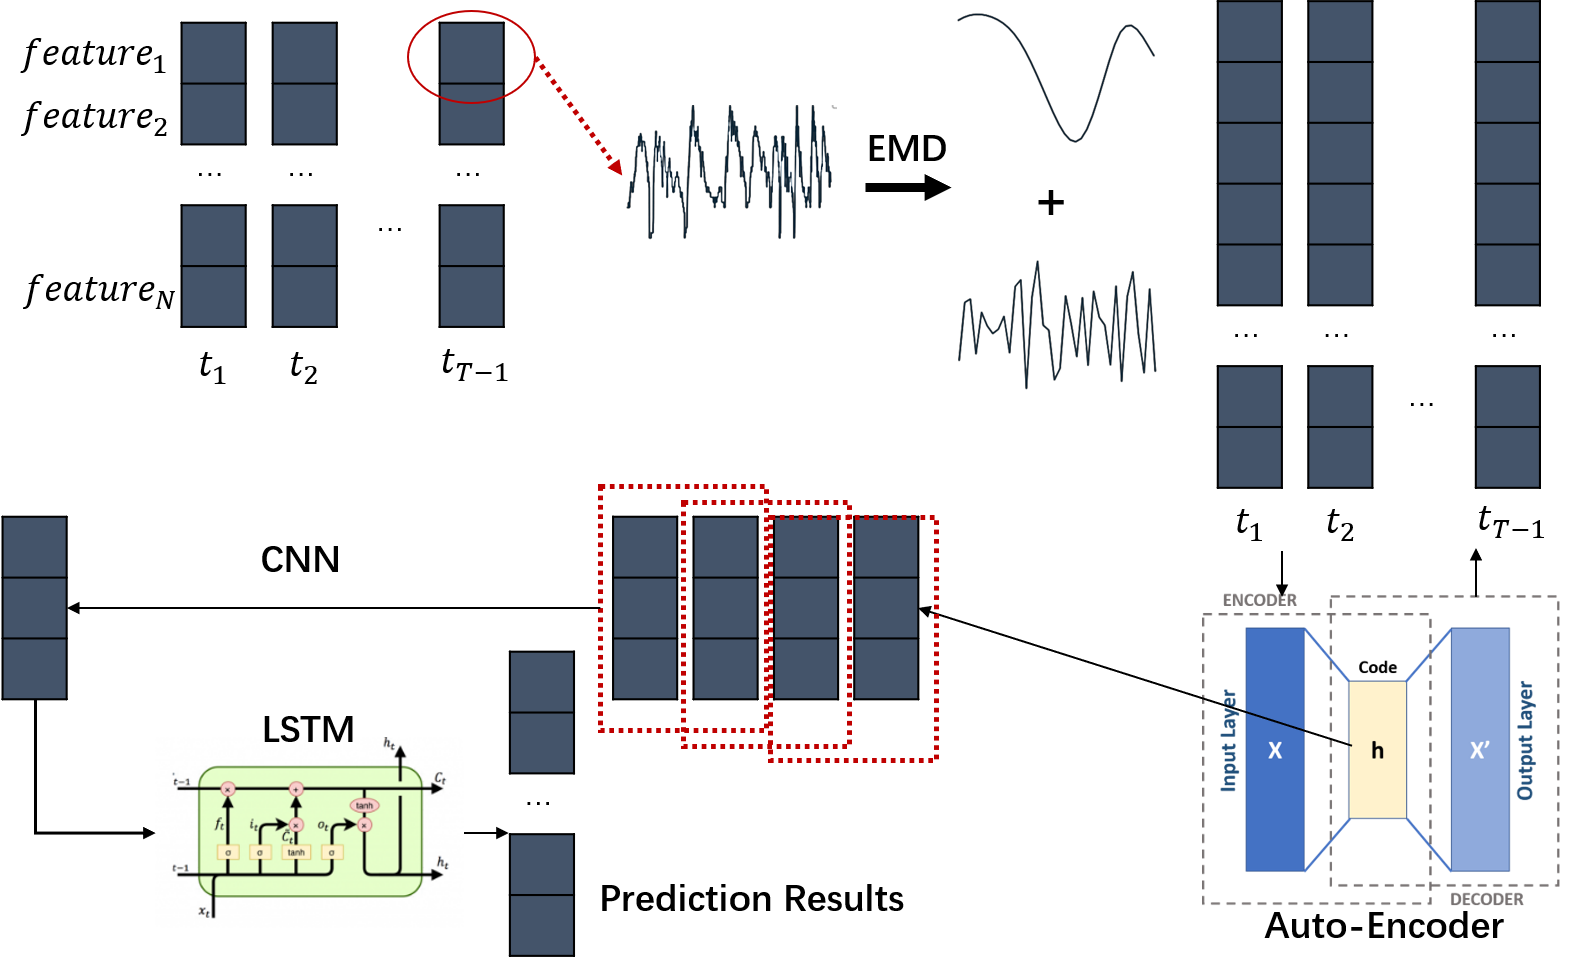
\includegraphics[width=\linewidth]{figures/prediction_system.png}
    \caption{工业装备状态预测部分系统设计}
    \label{fig:prediction system}
  \end{figure}

  如\ref{fig:prediction system}图中所示,这里给出了整体预测方案的系统设计方案。
  \begin{enumerate}
    \item 针对极值部分数据突变的预测技术。
    由于极值部分变化剧烈,往往预测效果不好。
    解决这个问题的一个方案就是对信号进行频率分解,
    这样输入的特征中会包含不同频率的信号特征,能够更好地预测极值部分的数据值。
    所以应用经验模态分解对时间序列进行信号处理,提取出不同频率的信号分量。
    \item 针对序列难建模的特点,提出应用CNN+LSTM组合的模型结构。
    \item 针对工业序列噪声大、特征之间相关程度高的特点,利用Auto-Encoder部分进行特征相关性的提取。
  \end{enumerate}
  

\subsection{方法说明}
在这一个小的章节中,将会对工业装备状态预测方案中采取的具体方法进行分别的说明。
\subsubsection{经验模态分解信号处理}
  \begin{figure}
    \centering
    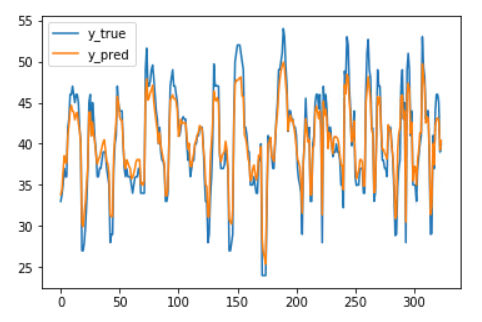
\includegraphics[width=0.8\linewidth]{figures/EMD动机.png}
    \caption{模型在高频处会预测效果差示意图}
    \label{fig:EMD motivation}
  \end{figure}
  通过实验观察发现,如图\ref{fig:EMD motivation}中所示的模型预测结果示意图
  (其中y\_true是真实值,y\_pred是预测值),
  模型预测结果的低频分量效果较好,
  但是容易在尖峰等轴温快速变化的位置预测效果相对较差。
  于是想通过EMD分解,可以提取不同频率的信号特征,进而提升模型预测效果。
  % Todo: EMD效果
\subsubsection{对高低频数据不同采样频率}
  为了进一步优化模型,在简单EMD方法的基础上,又进行了一些改进。
  由于EMD方法会将数据分解成多个不同的频率的数据,
  对于低频数据,采样太过密集会导致数据过于冗余,
  而对于高频数据,采样过于稀疏会导致高频部分数据失真。
  所以很容易想到,我们可以对不同频率的数据在输入模型前进行不同的采样频率的处理,
  在减少特征维度的同时,尽可能地提升数据的质量和模型预测效果。

\subsubsection{使用Layer Normalizaiton}
需要注意的是,由于后续需要利用重要性采样进行训练加速,为了统一,
模型中统一使用Layer Normalizaiton取代Batch Normalization。
这是因为,在重要性采样中会根据样本的重要性进行采样,
那么一个batch的样本不再是从原分布中随机产生,
不再满足和同分布的特点,那么Batch Normalization对于不同的batch的效果将不会是一致的。
会导致训练出现问题。

\subsubsection{不同时间序列预测的模型方案对比}
本文对比了几种不同模型在实验数据上的预测效果,下面分别介绍这几种模型的结构。

本文被用来对比的实验基准网络是一个全连接网络,

本文实现了长短时记忆网络,

通过实验测试了这几种不同网络的实际效果,
\subsubsection{自编码器在特征提取上的应用}
以上考虑了多个时间步上特征提取的模型结构问题,
但是在单个时间步上的多个特征之间,可能存在很强的相关性,
而特征的相互关系并不能用以上的模型结构表述,需要进一步处理。
这里提出利用Auto-Encoder结构捕捉特征之间的相关性。

需要注意的是,Auto-Encoder不需要完整地嵌入网络中,
只用将Encoder部分加入预测网络中,将Encoder的输出值输入其余部分的网络。
而且,这部分的网络无需参与后续的整个网络的梯度更新过程,只需要单独进行训练。

应用自编码器主要有两方面的目的,一方面自编码器自带的结构特征可以用来进行特征提取和降维,
另外一方面,自编码器具有降噪的效果,工业装备状态数据是实际采集到的数据,难免会存在很多噪声,
通过自编码器的应用,能够有效地减少噪声对模型的干扰。

那这里为什么选择用自编码器来进行降维,和常用的降维方法例如PCA
(Principal component analysis,主成分分析)方法对比。
PCA 方法只适用于线性降维,其他的降维方法也会受到数据的局限性,
但是自编码器降维的好处是利用深度神经网络来进行建模,对数据的拟合能力很强。
但是,自编码器降维在数据量比较小的时候容易出现过拟合的问题,
所以相对于PCA 方法而言,自动编码器更适用于复杂的大型数据集。
本论文讨论的主要针对工业装备状态这种长时间数据,采集到的数据很多,所以不用担心过拟合的问题。
% \paragraph{自编码器相关性处理}~{}
\paragraph{自编码器效果}~{}

通过实验我们发现,不是所有的工业装备状态预测的数据都适合用自编码器在特征维度进行降维。
例如在火车走行部的轴温预测中,各个不同的轴的温度会同步变换,
之间有比较强的相关性,而且这种相关性独立地存在于当前各个轴的温度状态中,
不需要额外的历史信息,解码器就能恢复出数据。

所以判断是否能够应用自编码器进行特征提取,我们可以通过训练的自编码器的输入和输出的比较,
如果差别比较小,说明编码器部分的信息损失比较小。

当然当出现自编码器效果不好时,也可以通过尝试别的不同结构的自编码器进行处理,
例如这里可以尝试编码器和解码器都是更加适用于序列处理的网络结构,例如LSTM模块,
但是在这里不作过多展开和研究。
\subsubsection{防止过拟合的策略}
针对在\ref{subsection_diffrent_divide}中提出的,
在序列化的划分方式下出现的过拟合问题,采用了加dropout的方式进行解决。
在后面应用LSTM时,也采用了同样的加dropout方式,同样也不存在过拟合问题。

\subsection{两种不同的状态预测方法}
对于状态预测有两种方式,一种是通过历史数据回归,
另外一种是结合历史数据和当前的其他可获得的电气信号预测。
这两种预测方式都有其各自的特点和适用的应用场景。

第一种通过历史数据回归的状态预测方法,它的应用场景更为广泛,
第二种需要获得当前的其他电气信号,有的场景下受到传感器数据收集速度或者数据传输速度的限制,
即时的信号并不那么容易获取,第一种方法就不会有这样的限制。

但是第一种方法也会存在相应的问题,有的时候会发生工况等状态的变化,
这样情况下简单通过历史的信息回归信息是不完备的。

\section{实验结果}

\subsection{往前预测多步结果}

  \begin{figure}
    \centering
    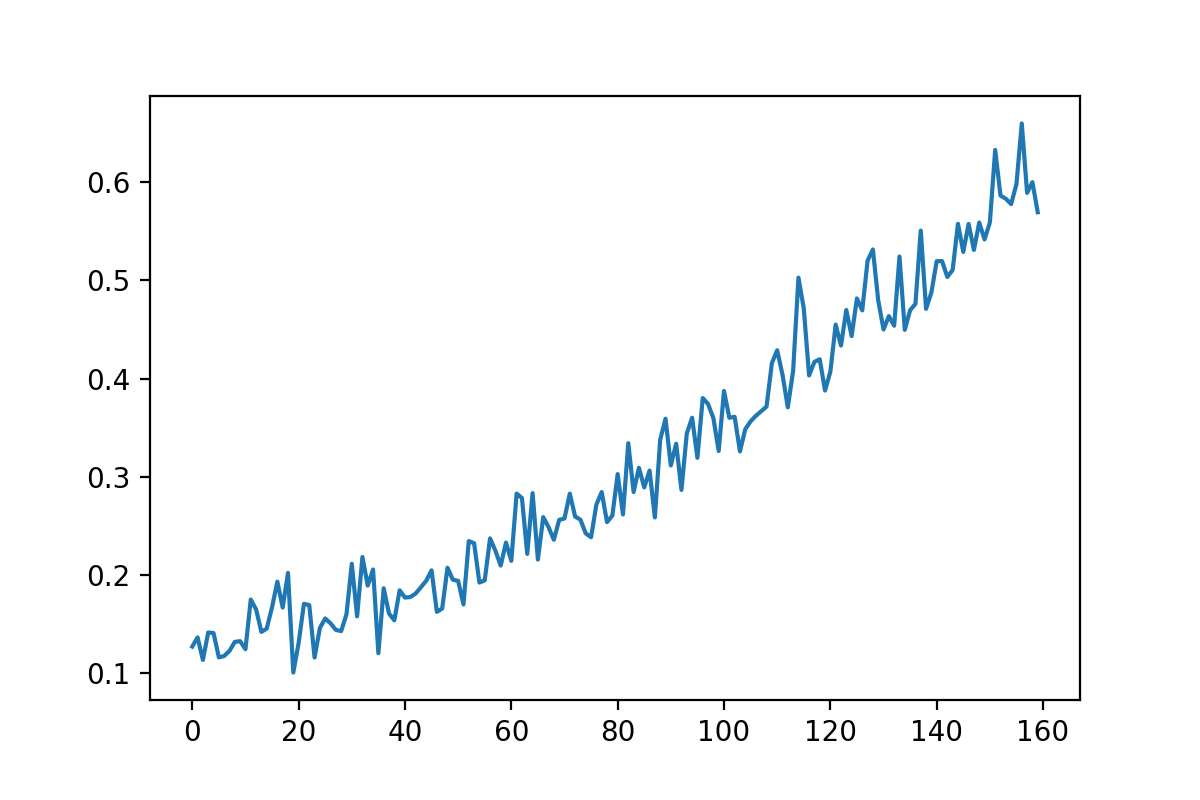
\includegraphics[width=0.8\linewidth]{figures/往前预测多步均方误差.png}
    \caption{往前预测多步均方误差(横轴坐标值代表往前预测的步数,纵轴是均方误差)}
    \label{fig:multi-step}
  \end{figure}

  预测的效果和设定的往前预测的时间长度相关。
  自回归往前预测第i步(i取1-160)的均方误差如图\ref{fig:multi-step}中所示,
  可以看到,往前预测得越远,均方误差越大,预测效果越差。
\subsection{防止过拟合的策略实验结果}

  \begin{figure}
    \centering
    \includegraphics[width=0.5\textwidth]{20210327_1505/FC losses.png}
    \caption{出现过拟合问题的网络训练过程loss变化}
    \label{fig:overfit FC 1}
  \end{figure}

  \begin{figure}
    \centering
    \begin{subfigure}[b]{0.45\textwidth}
      \centering
      \includegraphics[width=\textwidth]{20210327_2017/FC losses.png}
      \caption{FC losses with dropout}
      \label{fig:FC losses with dropout}
    \end{subfigure}
    \hfill
    \begin{subfigure}[b]{0.45\textwidth}
        \centering
        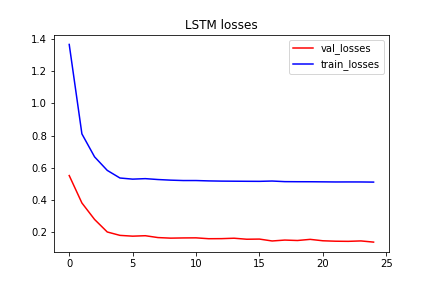
\includegraphics[width=\textwidth]{20210327_2017/LSTM losses.png}
        \caption{LSTM losses with dropout}
        \label{fig:LSTM losses with dropout}
    \end{subfigure}
       \caption{过拟合策略效果图:加了dropout之后的模型loss曲线变化}
       \label{fig:losses with dropout}
  \end{figure}

  如图\ref{fig:FC losses with dropout}中所示,
  对比前面图\ref{fig:overfit FC 1}中的结果,
  不再出现训练一段时间后训练集loss虽然一直在下降,但是验证集的loss反而再上升,
  而且训练集的效果远远好于测试集效果这样的情况。
  在模型过拟合方面有了明显改进。
  说明加dropout模块的方法十分有效。

\subsection{两种不同方法的工业装备状态预测的结果}
  
  \begin{table}
    \centering
    \caption{基于历史数据,150、192、222三组不同载荷下,电机温度预测均方误差结果}
    \begin{tabular}{lclcl}
      \toprule
      载荷       & 训练集MSE & 测试集MSE                                   \\
      \midrule
      150    & 0.357 & 0.334                                \\
      192 & 0.328 & 0.358                                     \\
      222 & 0.197 & 0.190                  \\
      \bottomrule
    \end{tabular}
    \label{tab:regression motor results}
  \end{table}

  \begin{table}
    \centering
    \caption{基于历史数据,150、192、222三组不同载荷下,PU温度预测均方误差结果}
    \begin{tabular}{lclcl}
      \toprule
      载荷       & 训练集MSE & 测试集MSE                                    \\
      \midrule
      150    & 0.011 & 0.017                                \\
      192 & 0.020 & 0.022                                     \\
      222 & 0.038 & 0.037                 \\
      \bottomrule
    \end{tabular}
    \label{tab:regression PU results}
  \end{table}
  
  \begin{table}
    \centering
    \caption{基于电气信号,150、192、222三组不同载荷下,电机温度预测均方误差结果}
    \begin{tabular}{lclcl}
      \toprule
      载荷       & 训练集MSE & 测试集MSE                                   \\
      \midrule
      150    & 0.014 & 0.670                                \\
      192 & 0.004 & 0.034                                    \\
      222 & 0.042 & 1.925                 \\
      \bottomrule
    \end{tabular}
    \label{tab:prediction motor results}
  \end{table}

  \begin{table}
    \centering
    \caption{基于电气信号,150、192、222三组不同载荷下,PU温度预测均方误差结果}
    \begin{tabular}{lclcl}
      \toprule
      载荷       & 训练集MSE & 测试集MSE                                    \\
      \midrule
      150    & 0.001 & 0.031                                \\
      192 & 0.004 & 0.032                                     \\
      222 & 0.026 & 0.610              \\
      \bottomrule
    \end{tabular}
    \label{tab:prediction PU results}
  \end{table}
  
  下面对两种不同方法分别进行实验,每种方法分别应用到电机温度预测和PU温度预测两个场景下,
  给出了在三种不同载荷情况下,训练集的MSE和测试集的MSE的最终结果。

  
  \ref{tab:regression motor results}和\ref{tab:regression PU results}
  给出的是第一种方法--基于历史信息的预测方法的结果,
  \ref{tab:prediction motor results}和\ref{tab:prediction PU results}
  给出的是第二种方法--基于电气信号的预测方法的结果。

  通过上面的结果可以看到,基于电气信号的方法的训练集MSE明显更小,而且差别比较悬殊,差了10倍以上,
  说明这样的方法的确提供的信息更完备。

  但是测试集的效果却反而不是很好,在基于电气信号的方法中,
  虽然数据提供的信息量更多,但是模型效果反而更差。
  分析原因是因为过拟合导致的,数据中的噪声也会导致这样的问题,加上MSE的数值本身就容易受到个别异常点的影响,
  所以导致了测试集MSE的结果比较差。



\section{本章小结}
在本章中讨论了关于工业装备状态预测的相关问题,
主要目标是搭建一个预测效果好的深度神经网络模型,
对不同的模型结构进行了研究和对比,同时提出了一些提高模型预测效果的方案。
